\begin{frame}[t,fragile]{自動微分(後退モード)}
  \begin{itemize}
    %\setlength{\itemsep}{1em}
  \item 次に上から順番に連鎖律を適用
    \begin{itemize}
    \item $\frac{\partial f}{\partial v_5} = d_{f,v_5} = -\frac{1}{4}$
    \item $\frac{\partial f}{\partial v_4} = d_{f,v_4} = \frac{1}{2}$
    \item $\frac{\partial f}{\partial v_3} = \frac{\partial f}{\partial v_4} \frac{\partial v_4}{\partial v_3} +  \frac{\partial f}{\partial v_5} \frac{\partial v_5}{\partial v_3}  = d_{f,v_4} d_{v_4,v_3} + d_{f,v_5} d_{v_5,v_3} = \frac{1}{2} \cdot 1 -\frac{1}{4} \cdot 1 = \frac{1}{4}$
    \item $\frac{\partial f}{\partial v_2} = \frac{\partial f}{\partial v_4} \frac{\partial v_4}{\partial v_2} = d_{f,v_4} d_{v_4,v_2} =  \frac{1}{2} \cdot 1 = \frac{1}{2}$
    \item $\frac{\partial f}{\partial v_1} = \frac{\partial f}{\partial v_2} \frac{\partial v_2}{\partial v_1} +  \frac{\partial f}{\partial v_3} \frac{\partial v_3}{\partial v_1} = d_{f,v_2} d_{v_2,v_1} + d_{f,v_3} d_{v_3,v_1} = \frac{1}{2} \cdot (-1) + \frac{1}{4} \cdot 1 = -\frac{1}{4}$
    \item $\frac{\partial f}{\partial x_3} = \frac{\partial f}{\partial v_3} \frac{\partial v_3}{\partial x_3} = \frac{1}{4} \cdot 1 = \frac{1}{4}$
    \item $\frac{\partial f}{\partial x_2} = \frac{\partial f}{\partial v_1} \frac{\partial v_1}{\partial x_2} = -\frac{1}{4} \cdot 1 = -\frac{1}{4}$
    \item $\frac{\partial f}{\partial x_1} = \frac{\partial f}{\partial v_2} \frac{\partial v_2}{\partial x_1} = d_{f,v_2} d_{v_2,x_1} = \frac{1}{2} \cdot 1 = \frac{1}{2}$
    \end{itemize}
  \item 計算の過程で、全ての独立・中間変数に関する偏導関数が自動的に求まる
  \item 計算量は$f$の値を計算するコストの定数倍

    % \vspace*{-10em} \hfill \resizebox{.3\textwidth}{!}{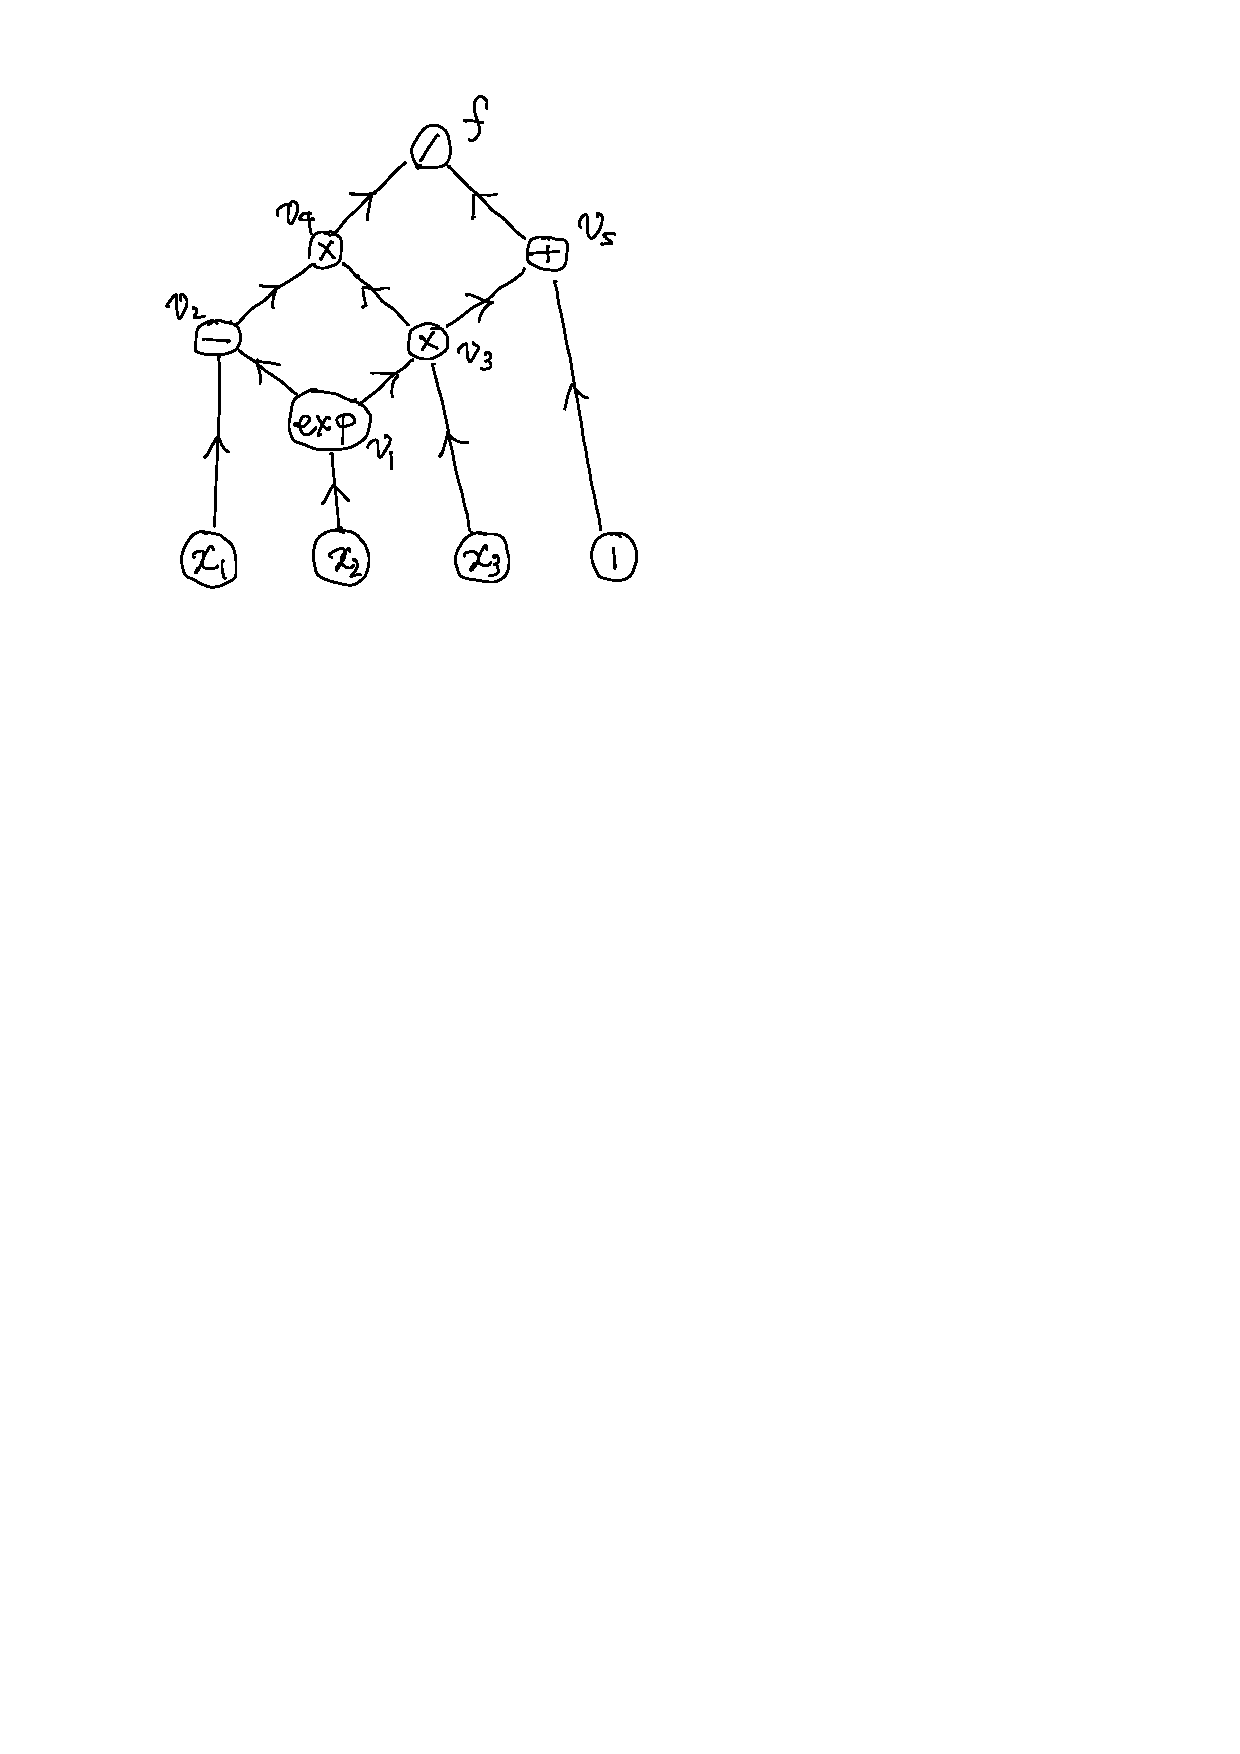
\includegraphics{image/compgraph.pdf}}
  \end{itemize}
\end{frame}
